% **************************************************
% Macro specifiche per il documento corrente
% **************************************************
% Nome
\newcommand{\docName}{Manuale Utente}
% Nome file
\newcommand{\docFileName}{manuale\_utente.2.0.pdf}
% Versione
\newcommand{\docVers}{2.0}
% Data creazione
\newcommand{\creationDate}{2013-02-22}
% Data ultima modifica
\newcommand{\modificationDate}{2013-05-16}
% Stato in {Approvato, Non approvato}
\newcommand{\docState}{Approvato}
% Uso in {Interno, Esterno}
\newcommand{\docUsage}{Esterno}
% Destinatari da specificare come nome1\\ &nome2\\ ecc.
\newcommand{\docDistributionList}{Prof. Tullio Vardanega\\ & Prof. Riccardo Cardin}
% Redattori da specificare come nome1\\ &nome2\\ ecc.
\newcommand{\docAuthors}{Riccardo Tresoldi}
% Approvato da
\newcommand{\approvedBy}{Marco Schivo}
% Verificatori
\newcommand{\verifiedBy}{Andrea Rizzi}
% Perscorso (relativo o assoluto) che punta alla directory contenente shared/
% come sua sottodirectory (per comodità chiamiamola 'doc root').
\newcommand{\docRoot}{..}
% definire se si vuole l'indice delle tabelle
\def\INDICETABELLE{false}
% definire se si vuole l'indice delle figure
\def\INDICEFIGURE{true}

% importa il preambolo condiviso da tutti i documenti
% shared/preamble.tex
%
% Questo documento contiene la parte del preambolo condivisa e viene pertanto
% richiamato nel 'master' di tutti i documenti di progetto.  Al suo interno
% contiene le inclusioni (e le configurazioni) di tutti i package richiesti per
% la compilazione dei documenti, le macro di carattere generale e la definizione
% degli stili di pagina.

\documentclass[a4paper,10pt,openright]{article}

% **************************************************
% Macro generiche
% **************************************************
\newcommand{\team}{Software Synthesis}                    % chi siamo
\newcommand{\email}{software.synthesis@gmail.com}         % e-mail
\newcommand{\caName}{}                                    % titolo capitolato
\newcommand{\caDescr}{}                                   % descrizione
\newcommand{\inglese}[1]{\textit{#1}}

% **************************************************
% Codifica e lingua dei documenti
% **************************************************
\usepackage[utf8x]{inputenc}                              % codifica caratteri dei documenti sorgenti
\usepackage[english,italian]{babel}                       % localizzazione ai fini di sillabazione e cross-references
\usepackage[T1]{fontenc}                                  % codifica font di output

% **************************************************
% Definizione geometria della pagina
% **************************************************
\usepackage[a4paper,head=4cm,top=4.5cm,bottom=3cm,left=3cm,right=3cm,bindingoffset=5mm]{geometry}

% *************************************************
% Intestazioni e piè di pagina personalizzati
% *************************************************
\usepackage{fancyhdr}
% stile normale
\fancypagestyle{normal}{
\fancyhead{}                                              % intestazione
\fancyhead[RE,RO]{
\begin{picture}(0,0)
  \put(-410,0){
\includegraphics[width=1.02\textwidth]{header_logo}}
  \put(-410,10){\sffamily\large\leftmark}
\end{picture}
\vspace{-4pt}
}
\renewcommand{\headrulewidth}{.4pt}                       % riga sotto l'intestazione
\cfoot{}                                                  % piè di pagina
\fancyfoot[RO,LE]{\sffamily
  pag.~\thepage{} di \pageref{LastPage}}                  % a dx nelle pag. dispari e a sx in quelle pari
\fancyfoot[RE,LO]{\sffamily\docFileName{} -- v.\docVers}
\renewcommand{\footrulewidth}{.4pt}                       % riga sopra il piè di pagina
}
% stile per gli indici
\fancypagestyle{toc}{
\fancyhead{}                                              % intestazione
\fancyhead[RE,RO]{
\begin{picture}(0,0)
  \put(-410,0){
\includegraphics[width=1.02\textwidth]{header_logo}}
\end{picture}
}
\renewcommand{\headrule}{}                                % nessuna riga sotto l'intestazione
\cfoot{}                                                  % piè di pagina
\fancyfoot[RO,LE]{\sffamily\thepage{}}                    % a dx nelle pag. dispari e a sx in quelle pari
\fancyfoot[RE,LO]{\sffamily\docFileName{} -- v.\docVers}
\renewcommand{\footrulewidth}{.4pt}                       % riga sopra il piè di pagina
}

\pagestyle{fancy}                                         % premetto: non so usare bene le marche:
\renewcommand{\sectionmark}[1]{\markboth{#1}{#1}}         % se qualcuno ha idee migliori si faccia avanti!

% **************************************************
% Tabelle
% **************************************************
\usepackage{tabularx}                                     % tabelle di larghezza fissa con una o più colonne variabili
\usepackage{multirow}                                     % colonne con colonne che si estendono per più righe
\usepackage{booktabs}                                     % per inserire l'ambiente table e le righe orizz. nelle tabelle
\usepackage{longtable}			                          % tabelle oltre i limiti di pagina

% **************************************************
% Cross-references e collegamenti ipertestuali
% **************************************************
\usepackage[hidelinks]{hyperref}
\hypersetup{%
  colorlinks=false, linktocpage=false, pdfborder={0,0,0}, pdfstartpage=3, pdfstartview=FitV,%
  urlcolor=Cyan, linkcolor=Cyan, citecolor=Black, %pagecolor=Black,%
  pdftitle={\docName}, pdfauthor={\team}, pdfsubject={}, pdfkeywords={},%
  pdfcreator={pdflatex}, pdfproducer={pdflatex with hyperref package}%
}

% **************************************************
% Immagini e grafica
% **************************************************
\usepackage{graphicx}                                     % supporto ad aspetti avanzati delle immagini
\graphicspath{{\docRoot/pics/}}                           % percorso contenente tutti i file immagini
\usepackage{color}                                        % permette di colorare facilmente il testo

% **************************************************
% Altri pacchetti opzionali
% **************************************************     
\usepackage{lastpage}                                     % per sapere il numero totale di pagine
\usepackage{lipsum}                                       % genera "dummy text" per prove di impaginazione
\usepackage{eurosym}                                      % per il simbolo dell'euro usare \EUR{x} dove x è l'importo


\usepackage[italian]{varioref}

% Fine del preambolo e inizio del documento
\begin{document}

% Inclusione della prima pagina
% shared/firstpage.tex
%
% Questo documento definisce il contenuto della prima pagina, che si suppone
% essere uguale in tutti i documenti.  Oltre al logo e al titolo, la prima
% pagina contiene i metadati relativi al documento in cui viene inclusa.


% rimuove intestazioni e piè di pagina
\pagestyle{empty}

\begin{center}

% logo del gruppo

\includegraphics[width=1.5\textwidth]{logo}

\vspace{1in}

% titolo del documento
{\Huge\bfseries \docName}

\vspace{1in}

% tabella riepilogativa
\begin{tabularx}{.7\textwidth}{>{\bfseries\sffamily}l>{\sffamily}l}
\toprule
\multicolumn{2}{>{\sffamily}c}{Informazioni sul documento}\\
\midrule
Nome file:            & \docFileName\\
Versione:             & \docVers\\
Data creazione:       & \creationDate\\
Data ultima modifica: & \modificationDate\\
Stato:                & \docState\\
Uso:                  & \docUsage\\
Redattori:            & \docAuthors\\
Approvato da:         & \approvedBy\\
Verificatori:         & \verifiedBy\\
\bottomrule
\end{tabularx}

\end{center}

\newpage


% Storico delle modifiche
\section*{Storia delle modifiche}
\begin{longtable}{lp{.3\textwidth}lll}
\toprule
Versione & Descrizione intervento & Redattore & Ruolo & Data\\
\midrule % inserire qui il contenuto della tabella

2.0 & Approvato documento & Marco Schivo & Responsabile & 2013-05-16\\
1.4 & Verificato documento & Andrea Rizzi & Verificatore & 2013-05-16\\
1.3 & Corretta descrizione della home dell'applicativo & Riccardo Tresoldi & Verificatore & 2013-05-16\\
1.2 & Descritte nuove funzionalità non implementate nella versione 1.0 & Stefano Farronato & Verificatore & 2013-05-16\\
1.1 & Aggiornate le immagini-screen dell'interfaccia grafica. & Riccardo Tresoldi & Verificatore & 2013-05-16\\
1.0 & Approvazione del documento. & Andrea Rizzi & Responsabile & 2013-03-25\\
0.5 & Verifica lessico ortografica del documento. & Diego Beraldin & Verificatore & 2013-03-24\\
0.4 & Inserito glossario e \textit{screen} delle schermate dell'applicazione.& Stefano Farronato & Verificatore & 2013-03-23\\
0.3 & Stesura istruzioni per l'uso e completamento sezione relativa alle istruzioni per l'accesso. & Stefano Farronato & Verificatore & 2013-03-23\\
0.2 & Stesura istruzioni per l'accesso & Stefano Farronato & Verificatore & 2013-03-22\\
0.1 & Stesura scheletro documento e introduzione. & Elena Zecchinato & Programmatore & 2013-03-22\\
\bottomrule
\end{longtable}
\newpage

% inclusione dell'indice
% shared/toc.tex
%
% Questo file contiene le istruzioni che generano l'indice o gli indici del
% documento (utile nel caso in cui decidessimo di avere anche un indice delle
% tabelle e/o un indice delle figure).

\pagestyle{toc}
\pagenumbering{roman}

\tableofcontents

\newpage



% Alcuni aggiustamenti per le pagine
\pagenumbering{arabic}
\setcounter{page}{1}
\pagestyle{normal}

% Qui ha inizio il documento vero e proprio...
\section{Introduzione}
\subsection{Scopo del prodotto}
Il prodotto ``MyTalk'' è un sistema software di comunicazione tra utenti mediante \underline{\inglese{browser}} internet, senza la necessità di installazione di \underline{plugin} e/o software esterni. Gli utenti avranno la possibilità di interagire mediante una comunicazione audio - audio/video - testuale e, inoltre, ottenere le statistiche sull'attività in tempo reale.

\subsection{Scopo del Manuale}
Lo scopo del presente manuale è quello di fornire una guida per comprendere e utilizzare al meglio l'applicazione ``\caName''.
Tale documento contiene la descrizione delle principali funzionalità del prodotto ed il modo
per utilizzarle.

\subsection{Destinatario del manuale}
L'applicazione  ``\caName'' è indirizzata agli utenti che desiderano effettuare una comunicazione audio/video/testuale tramite un computer in modo semplice  e senza dover installare nessun software esterno.  

\subsection{Come leggere il manuale}
Il manuale è un integrazione illustrativa e di supporto nell'uso dell'applicazione \caName{} e ha lo scopo di illustrarne le funzionalità nel modo più chiaro e semplice possibile, al fine di godere della massima gratificazione durante l'esperienza d'uso.

Il manuale è diviso essenzialmente in due parti, nella prima vengono descritte le istruzioni d'accesso, i requisiti del sistema,le modalità per riportare eventuali malfunzionamenti, la modalità di registrazione e l'autenticazione all'applicazione stessa. 
Nella seconda vengono descritte invece le varie funzioni che \caName{} offre: le modalità di comunicazione con gli altri utenti, l'interazione con la rubrica personale,la gestione del proprio \underline{\inglese{account}}, l'utilizzo della segreteria e la visualizzazione dello storico delle chiamate.

Al termine sarà inoltre riportato un breve glossario contenente i termini utilizzati in questo manuale e che potrebbero causare difficoltà all'utente nella comprensione del testo. Tali termini saranno contrassegnati tramite sottolineatura. 

\section{Istruzioni per l'accesso}

\subsection{Installazione}
L'applicazione non necessita di installazione, è sufficiente aprire il \inglese{browser}, selezionare la barra relativa all'inserimento dell'\underline{\inglese{url}} e digitare
\begin{center}
 \url{http://www.softwaresynthesis.org/MyTalk}
\end{center}
Una volta raggiunto il sito sarà possibile iniziare ad usufruire del prodotto senza ulteriori operazioni.

\subsection{Requisiti del sistema}
\subsubsection{Requisiti software}
Il corretto funzionamento del software ``\caName'' è assicurato solo con i seguenti \inglese{browser}:
\begin{itemize}
  \item Google Chrome (versione minima 23.0.1271.97m)
\end{itemize}

Tuttavia, pur utilizzando tali \inglese{browser} non è garantita la possibilità di controllo delle statistiche. Infatti, tale funzionalità attualmente è disponibile solo per la \underline{versione sviluppatori} dei \inglese{browser}, tuttavia molto probabilmente sarà possibile disporre di tali funzionalità offerte dall'applicativo nelle prossime (e imminenti) versioni degli stessi.
L'utente deve inoltre disporre delle seguenti risorse \inglese{hardware}, oltre allo scontato computer dell'utente:
\begin{itemize}
  \item connessione a internet;
  \item microfono e/o  \inglese{webcam}.
 \end{itemize}

\subsubsection{Prerequisiti}
All'utente non sono richieste conoscenze particolari oltre alla comune esperienza di navigazione web.

\subsection{Comunicare il rilevamento di problemi e malfunzionamenti}
Nell'eventualità in cui durante l'utilizzo del software \caName{} si dovessero riscontrare malfunzionamenti o comportamenti inattesi che non corrispondono a quanto descritto nel presente manuale, si invita ad inviare le proprie segnalazioni all'indirizzo:
\begin{center}
  \email{}
\end{center}
specificando le seguenti informazioni:
\begin{itemize}[noitemsep,nolistsep]
  \item[-] il \inglese{browser} utilizzato, la versione dello stesso e il sistema operativo;
  \item[-] una descrizione più dettagliata possibile del problema riscontrato e le circostanze in cui si è verificato;
  \item[-] i messaggi d'errore (e i codici associati) che sono stati presentati.
\end{itemize}

\subsection{Registrazione}
Qual'ora un utente desideri usufruire del servizi offerti dall'applicazione ``\caName'' dovrà effettuare la registrazione al sistema.\\
L'utente può accedere alla pagina registrazione premendo il pulsante \texttt{Registrazione} visualizzato in figura:

\begin{figure}[H]
  \centering
  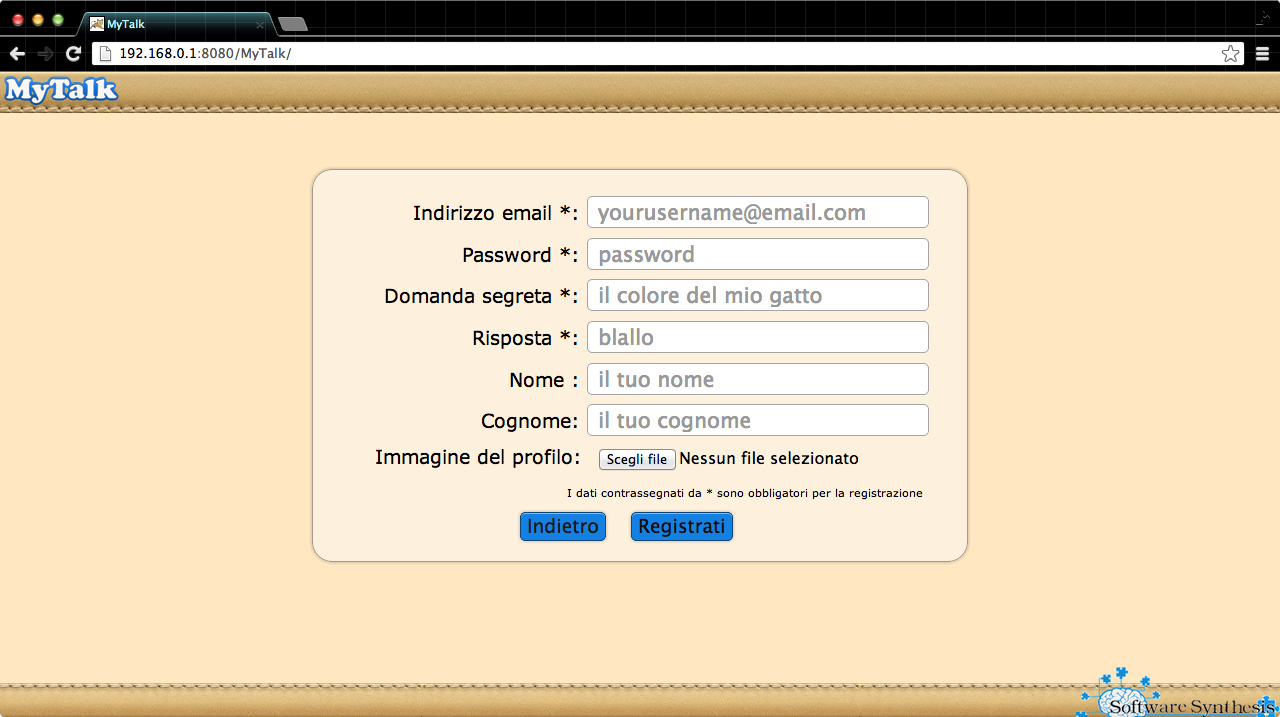
\includegraphics[width=0.85\textwidth]{manual_register}
\caption{Form di registrazione all'applicazione}\label{fig:register}
\end{figure}


Per effettuare la registrazione l'utente deve inserire obbligatoriamente uno \underline{\inglese{username}}, che corrisponderà alla sua mail, e una \inglese{password}.
L'utente per motivi di sicurezza deve inoltre scegliere una ``domanda segreta'' e fornirne la risposta a tale domanda, in modo che nel caso venga dimenticata la \inglese{password} si riesca a recuperarla, dopo aver superata questo vincolo di sicurezza.
Successivamente si potranno inserire alcuni dati facoltativi e atti al completamento informativo del proprio \inglese{account}: tra questi troviamo il nome, il cognome e l'immagine di profilo.

Ai fini di una maggiore sicurezza dell'autenticazione, il sistema fornirà una valutazione testuale sulla complessità della password scelta, visualizzabile a sinistra della \textit{form} di inserimento della stessa.

Una volta inseriti i dati richiesti e premuto il pulsante \texttt{Registrati} la registrazione sarà avvenuta e si verrà re-indirizzati alla pagina principale dell'allicazione.

\subsection{Autenticazione}
L'utente registrato al sistema ha la possibilità di autenticarsi al server \caName{} ed accedere al servizio, inserendo il suo \inglese{username} e la \inglese{password} associata.
Dopo un attesa di pochi secondi si verrà ri-indirizzati automaticamente alla schermata principale dell'applicazione, da dove è possibile raggiungere ogni servizio disponibile.

\begin{figure}[H]
  \centering
  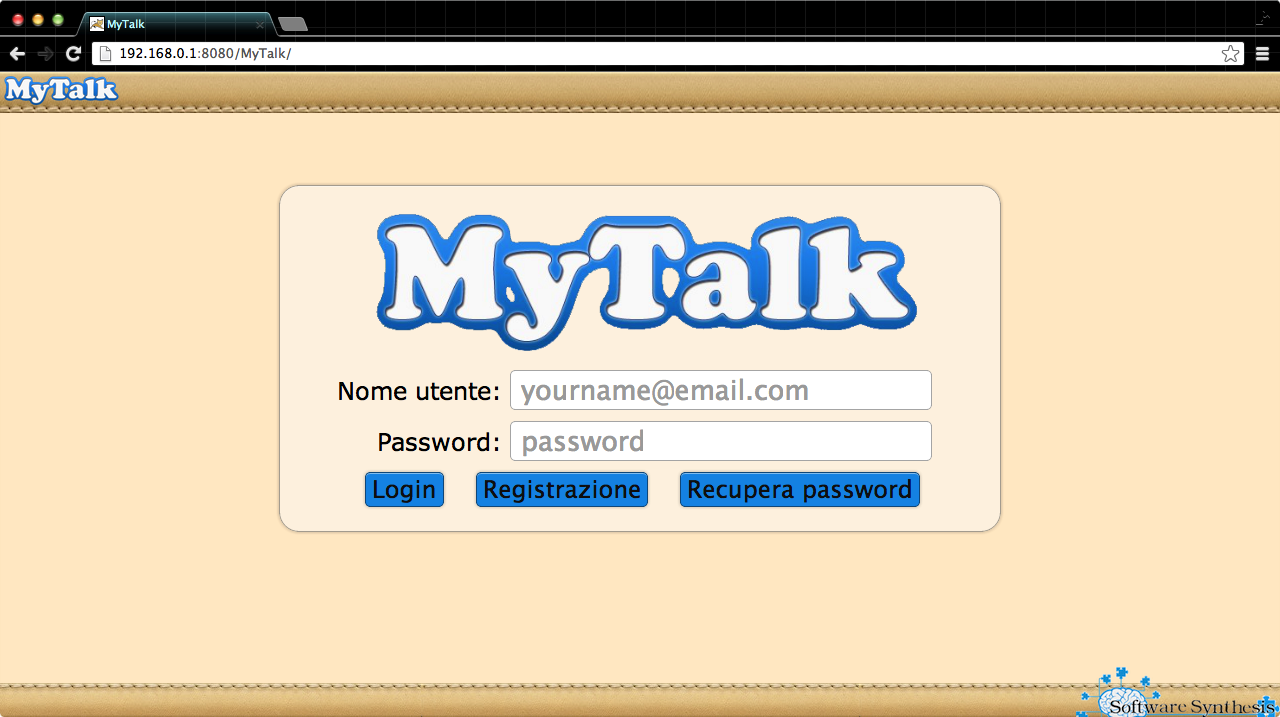
\includegraphics[width=0.85\textwidth]{manual_login}
\caption{Schermata di login all'applicazione}\label{fig:login}
\end{figure}

\subsection{Recupero Password}
Tramite il pulsante \texttt{Recupera password} è possibile recuperare la stringa scelta per autenticarsi al sistema. Nella schermata visualizzata sarà necessario inserire la risposta alla domanda segreta precedentemente impostata, una volta inserita correttamente verrà inviato al proprio indirizzo \texttt{mail} (che sarà identificato dal nome utente) la password smarrita per effettuare l'autenticazione.

\begin{figure}[H]
  \centering
  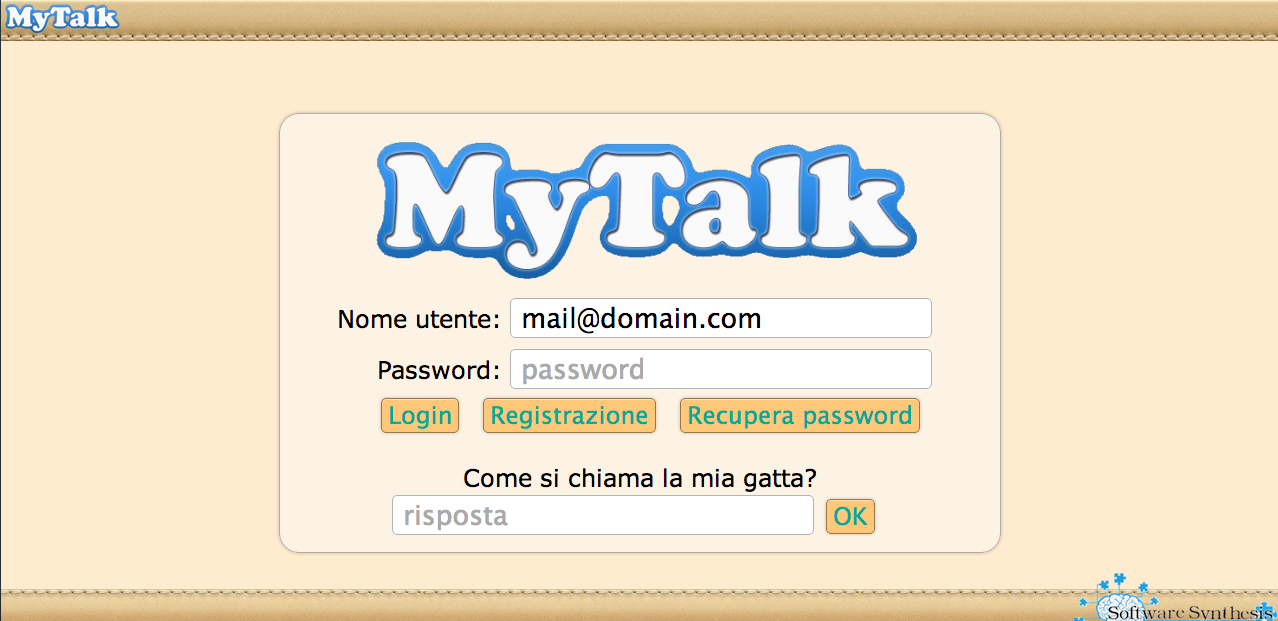
\includegraphics[width=0.85\textwidth]{manual_answer}
\caption{Schermata di recupero della password}\label{fig:answer}
\end{figure}


\section{Istruzioni per l'uso}
\subsection{Home Screen dell'applicativo }
La \underline{schermata Home} di \caName{} è caratterizzata essenzialmente da tre aree principali.

\begin{figure}[H]
  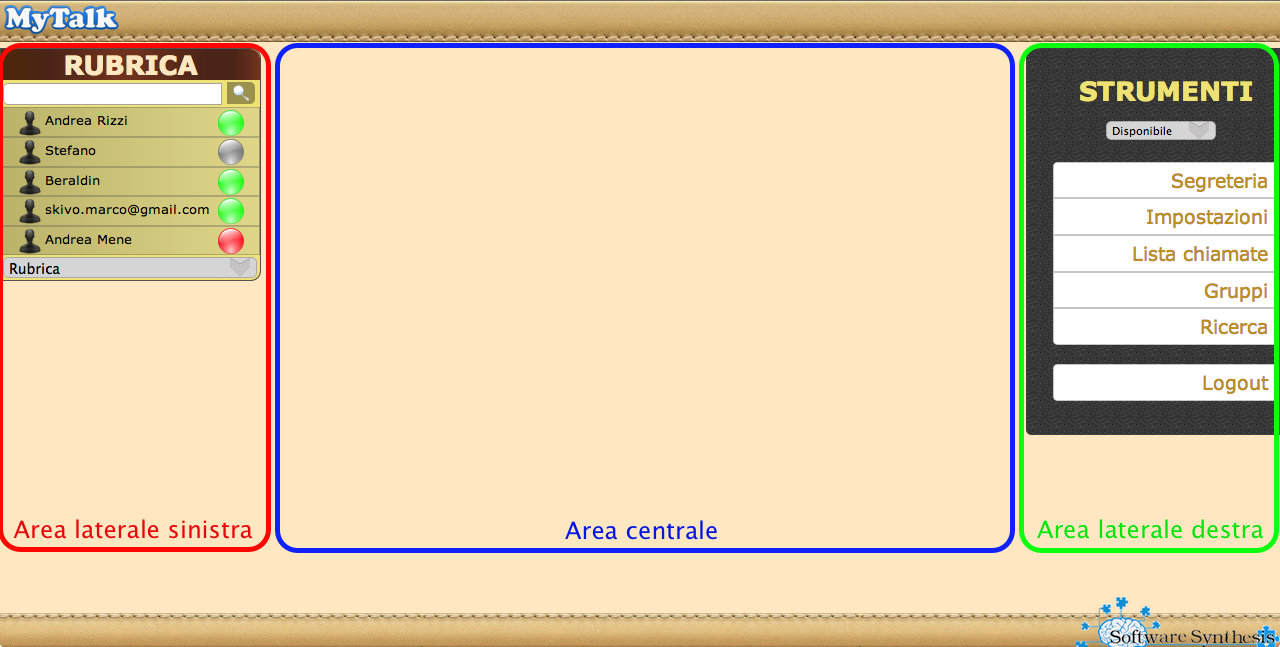
\includegraphics[width=\textwidth]{manual_main2}
\caption{Schermata principale}\label{fig:main}
\end{figure}


\begin{description}
\item \textcolor{blue}{\textbf{Area centrale:}} sarà visualizzabile ogni chiamata e/o interazione con un utente con cui si desidera comunicare nonché le varie finestre relative alla segreteria e alla visualizzazione del registro chiamate. Quest'area sarà in sostanza il fulcro dell'applicazione stessa, in quanto attraverso di essa vengono erogate tutte le modalità di comunicazione.

\item \textcolor{green}{\textbf{Area laterale destra:}} area dedicata ai servizi a disposizione dell'utente. È possibile accedere a tutte le funzionalità collegate alla gestione del proprio \inglese{account} che verranno successivamente espanse nell'area centrale descritta precedentemente:
\begin{description}
\item \textbf{Stato personale}: lo stato (\texttt{disponibile-occupato-non disponibile}) che verrà visualizzato dai contatti che hanno il nostro riferimento nella loro rubrica, è possibile impostarlo mediante il pratico menù a tendina.
\item \textbf{Segreteria}: viene visualizzata nell'area centrale la gestione della segreteria. Per maggiori informazioni sul suo utilizzo, rimandiamo il lettore alla sezione \texttt{3.7 Segreteria}.
\item \textbf{Impostazioni}: vengono visualizzate nell'area centrale le informazioni relative al 
proprio \inglese{account}, con la possibilità di effettuare eventuali modifiche ai campi dati. Il lettore potrà trovare un maggior contenuto informativo, in merito all'uso di tale funzionalità, nell'apposita sezione \texttt{3.6 Impostazioni Account}.
\item \textbf{Lista Chiamate}: viene visualizzata nell'area centrale la lista delle chiamate effettuate e ricevute in ordine cronologico (dalla più recente). La lista è provvista di elementi definiti nel seguente modo:
	\begin{itemize}
		\item il nome e il cognome (o \inglese{username} nel caso in cui il contatto fosse sprovvisto di nome e cognome) del chiamante o del chiamato (a seconda del caso);
		\item data ed ora ora in cui è iniziata la chiamata.
	\end{itemize}
	Inoltre le chiamate effettuate dall'utente saranno visualizzate su uno sfondo verde. Quelle ricevute invece saranno visualizzate su di uno sfondo rosso.
\item \textbf{Gruppi}: viene visualizzata nell'area centrale \inglese{form} per la creazione e l'eliminazione dei gruppi in cui vengono catalogati i contatti presenti nella rubrica.
\item \textbf{Ricerca}: visualizza nell'area centrale la \inglese{form} per la ricerca degli utenti. La ricerca consiste nell'inserimento di una parola chiave che verrà confrontata con il nome, il cognome e l'\inglese{username} degli utenti del sistema. Ogni utente che contiene (nei suddetti campi) la parola ricercata, verrà visualizzato in una lista sottostante alla \inglese{form} di ricerca.
\item \textbf{Chiamata}: voce che verrà a comparire solo se, durante una chiamata, decide di passare ad un'altra voce del menù laterale (e.g Impostazioni). Quando ciò accade, il contenuto dell'area centrale cambiare di contenuto (coerentemente con la voce selezionata), ma avendo comunque la possibilità di continuare a comunicare con l'utente chiamato (o chiamante). la pressione del pulsante chiamata gli permetterà di visualizzare nuovamente, nell'area centrale, il video della chiamata corrente.
\item \textbf{Logout}: permette all'utente di disconnettersi dall'applicativo.
\end{description}
\item \textcolor{red}{\textbf{Area laterale sinistra}} area dedicata alla rubrica dell'utente. In questo spazio è presente la lista degli utenti registrati nella rubrica dell'utente, dai quali sarà possibile avviare le operazioni di chiamata e (in generale) di visualizzazione dei profili degli stessi. L'approfondimento sulle funzionalità offerte da tale strumento, sarà trattato nella sezione \texttt{3.5 Rubrica}, di questa guida.
\end{description}

\clearpage

\subsection{Chiamata}
Per iniziare una chiamata audio è necessario selezionare dalla rubrica (o ricercando nel database generico) il contatto con cui si desidera comunicare. Nell'area centrale della pagina appariranno i dati dell'utente selezionato, e tramite un \inglese{click} sul pulsante \texttt{chiama} è possibile iniziare la chiamata con il suddetto utente.

\begin{figure}[H]
  \centering
  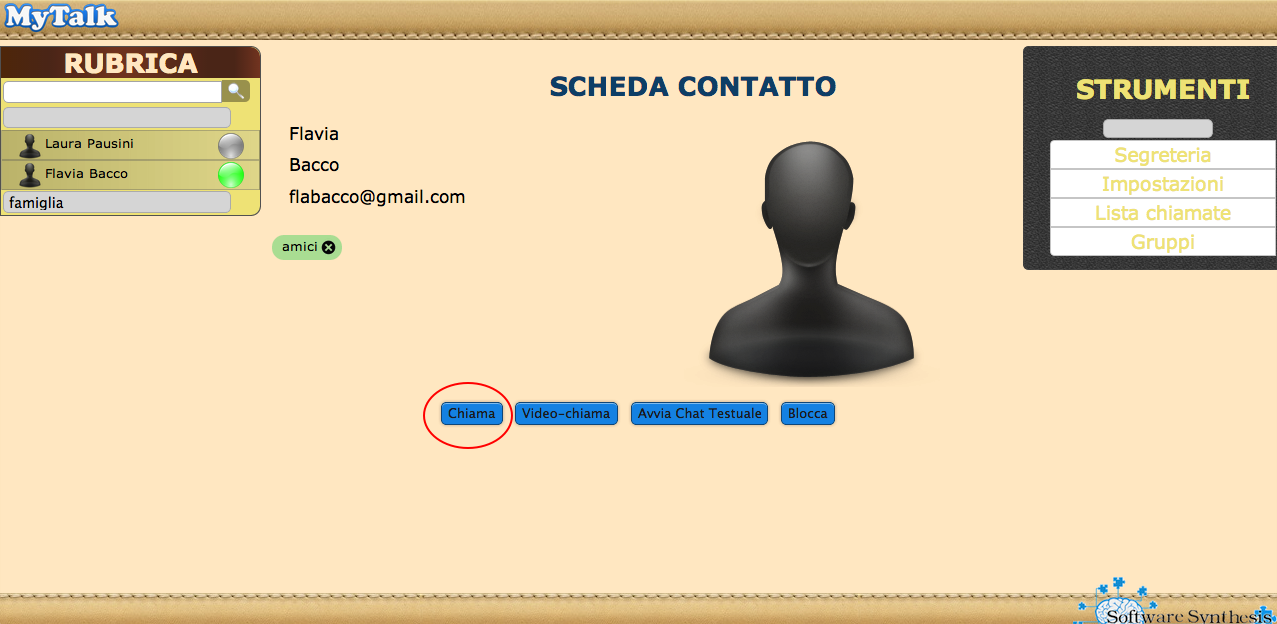
\includegraphics[width=0.85\textwidth]{manual_audioCall.png}
\caption{Schermata di selezione chiamata audio}\label{fig:audioCall}
\end{figure}

Una volta avviata la chiamata non sarà presente nessun elemento nella pannello centrale, confermando l'assenza dello \inglese{streaming} video dell'utente contattato. 
Nella parte inferiore del pannello centrale sono presenti invece la statistiche di utilizzo, quali i dati inviati e ricevuti e il tempo di comunicazione, e il pulsante per terminare la chiamata stessa.

\begin{figure}[H]
  \centering
  \includegraphics[width=0.85\textwidth]{manual_audioCall2.png}
\caption{Schermata comunucazione audio}\label{fig:audioCall2}
\end{figure}

\clearpage

\subsection{Video chiamata}
Per iniziare una chiamata audio video, analogamente alla chiamata audio, è necessario selezionare dalla rubrica (o ricercando nel database generico) il contatto con cui si desidera comunicare. Nell'area centrale della pagina appariranno i dati dell'utente selezionato, e tramite un \inglese{click} sul pulsante 
\texttt{video-chiama} è possibile iniziare la chiamata con il suddetto utente.

\begin{figure}[H]
  \centering
  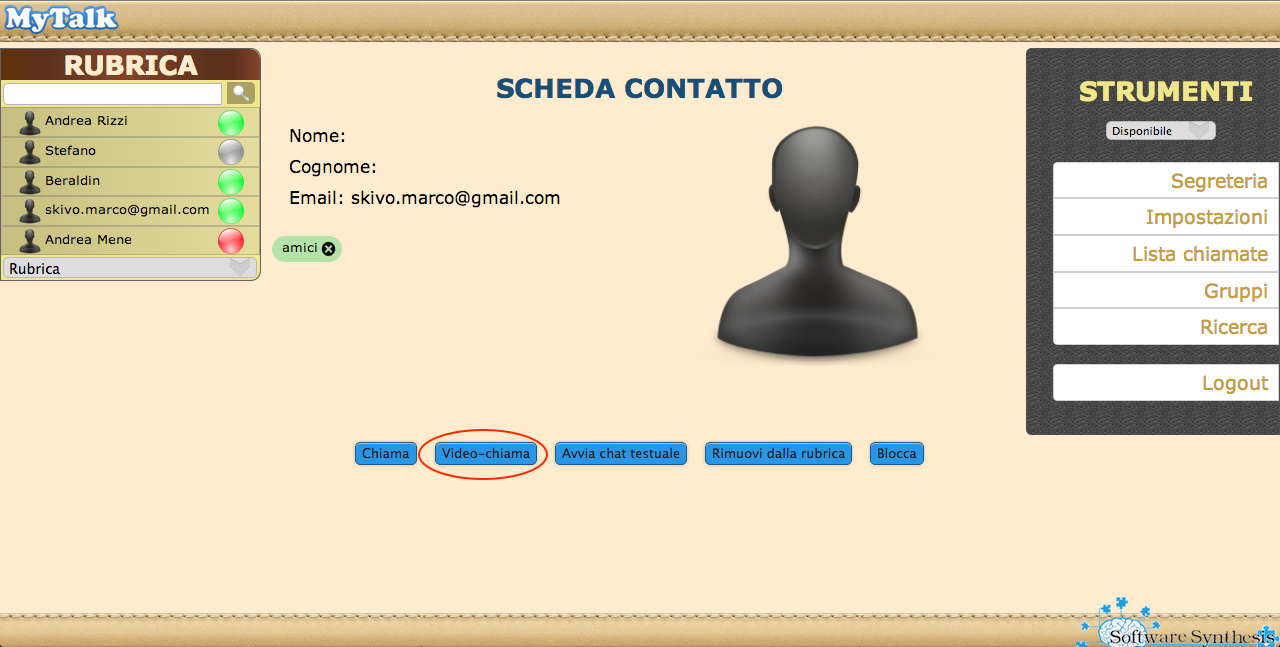
\includegraphics[width=0.85\textwidth]{manual_videoCall.png}
\caption{Schermata di selezione chiamata audio-video}\label{fig:videoCall}
\end{figure}

Una volta avviata la video-chiamata sarà visualizzata la \inglese{webcam} dell'utente da noi contattato, nonché un piccolo riquadro con rappresentata l'anteprima della \inglese{webcam} personale il cui flusso video è visibile all'utente con cui stiamo comunicando. 
Nella parte inferiore del pannello centrale è presente il pulsante per terminare la chiamata e la statistiche di utilizzo, quali i dati inviati e ricevuti e il tempo di comunicazione.

\begin{figure}[H]
  \centering
  \includegraphics[width=0.85\textwidth]{manual_videoCall2.png}
\caption{Schermata comunucazione audio-video}\label{fig:videoCall2}
\end{figure}

\clearpage
\subsection{Chat}
La \inglese{chat} testuale è disponibile con ogni utente contatto presente in rubrica e non necessita di ulteriori strumenti (microfono-webcam) da parte degli utenti coinvolti per essere avviata. Analogamente alle chiamate ``classiche'', anche per la \inglese{chat} è necessario selezionare dalla rubrica (o ricercando nel database generico)  il contatto con cui si desidera comunicare. Nell'area centrale della pagina appariranno i dati dell'utente selezionato, e tramite un \inglese{click} sul pulsante \inglese{chat} è possibile iniziare la conversazione testuale con il suddetto utente.\\

\begin{figure}[H]
  \centering
  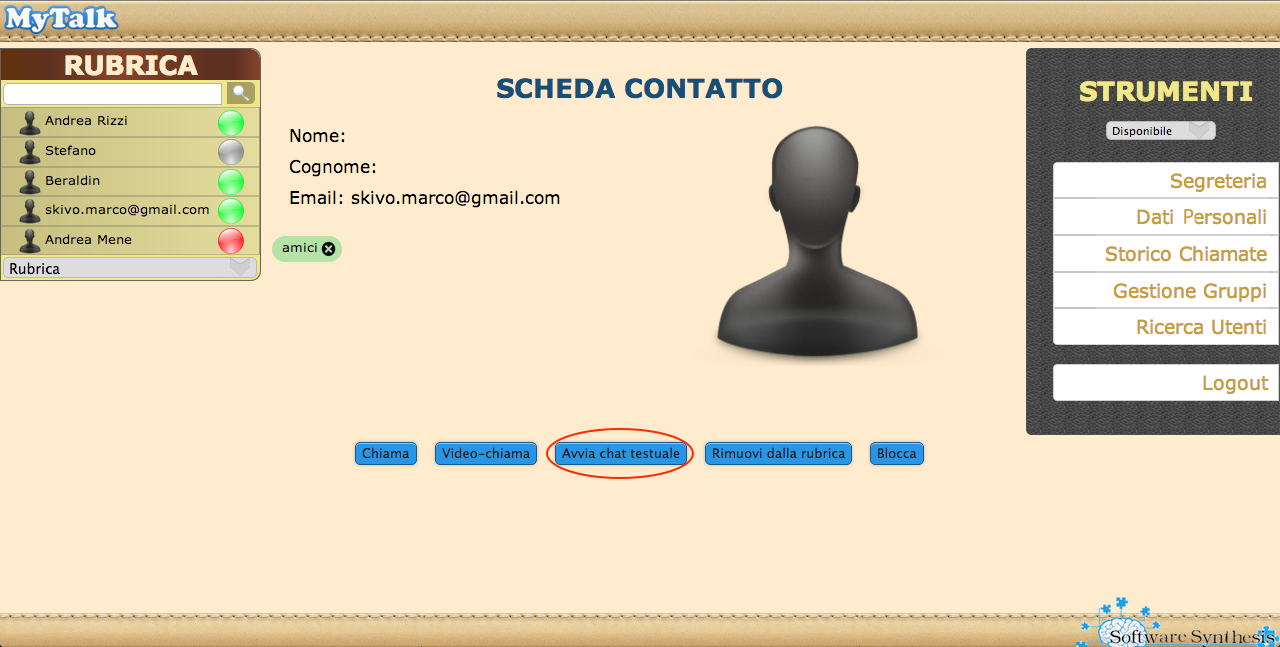
\includegraphics[width=0.8\textwidth]{manual_chat.png}
\caption{Schermata di selezione chat}\label{fig:chat}
\end{figure}

Il pannello di \inglese{chat} sarà quindi composto da due semplici sezioni rettangolari. Nella parte superiore è riportata la conversazione svolta sino ad ora tra i due utenti che aderiscono alla \inglese{chat}, mentre nella parte inferiore sarà possibile scrivere il messaggio da inviare successivamente (tramite il pulsante \texttt{invia} al contatto selezionato.\\
Premendo infine il pulsante ``\texttt{X}'' a destra del nome del contatto, si terminerà la comunicazione testuale in corso.

\begin{figure}[H]
  \centering
  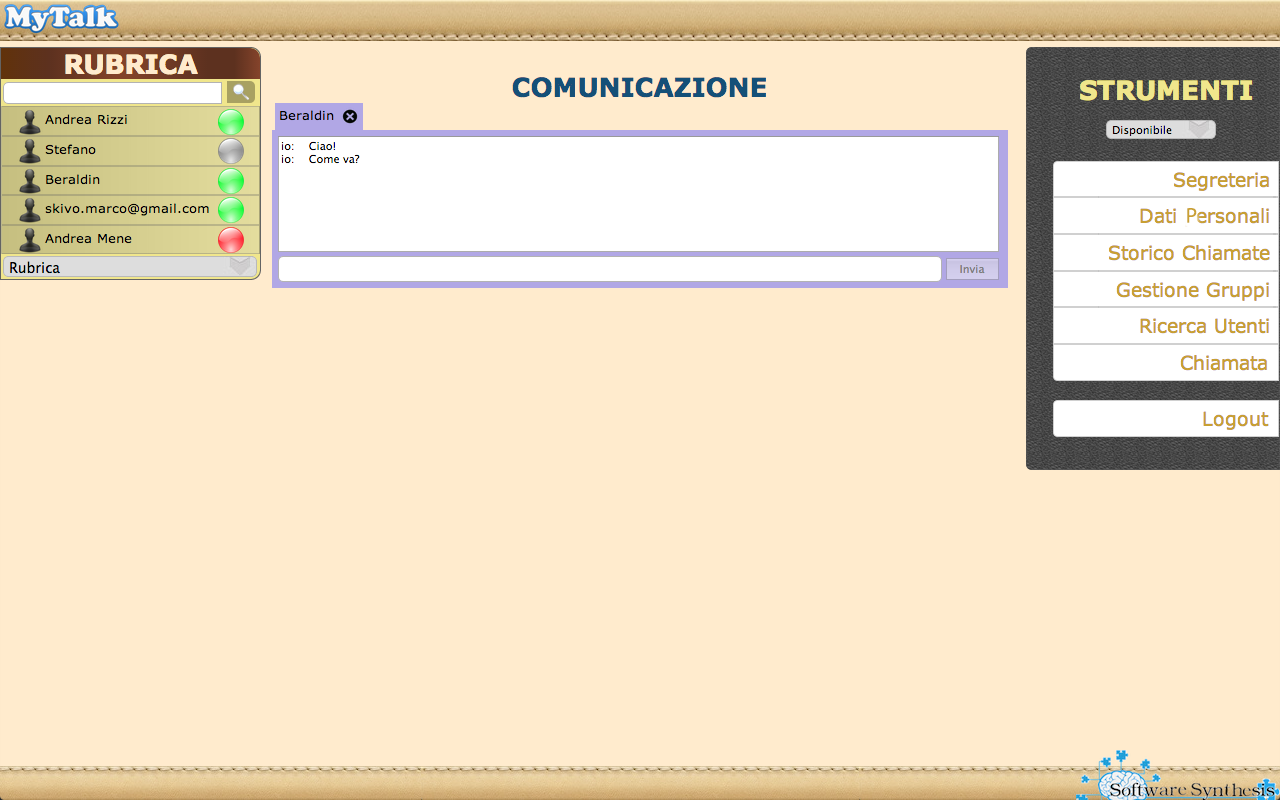
\includegraphics[width=0.8\textwidth]{manual_chat2.png}
\caption{Schermata comunucazione chat}\label{fig:chat2}
\end{figure}

\clearpage
\subsection{Rubrica}
Nella parte sinistra della schermata home di \caName{} è possibile visualizzare e interagire con i contatti presenti in rubrica, nonché eliminarli da essa, ciò avviene mediante la ricerca tra gli utenti iscritti al sistema nel pannello strumenti dell'utente, tramite il pulsante \texttt{Gestione contatti}.

Ogni contatto viene visualizzato con il proprio nome ed il proprio cognome, qual'ora tale contatto non avesse inserito i campi relativi al nome o al cognome (condizione legata all'opzionalità di tali in fase di registrazione), verrà visualizzato solo le informazioni di cui è provvisto il contatto (e.g un utente con nome Mario e cognome non impostato sarà visualizzato solo con il proprio nome). 
Nel caso non avesse impostato ne il nome ne il cognome, egli comparirà nella rubrica con il proprio \inglese{username}. 
Ogni contatto è inoltre provvisto di un'immagine utente e di un icona ''notifica di presenza''. Tale icona viene usata per comunicare all'utente la sua disponibilità (icona di notifica verde) o l'impossibilità a comunicare (icona di notifica rossa). L'icona diventerà grigia se il contatto visualizzato non è attualmente in linea.

È inoltre disponibile una pratica \inglese{form} di ricerca per contatti, la possibilità di ordinare la lista in base a determinate regole organizzative, e di visualizzare gli utenti filtrandoli per gruppi nei qualis sono inseriti tramite l'apposito pulsante disponibile nell'area dedicata ai servizi a disposizione dell'utente.

\clearpage
\subsection{Segreteria}
La segreteria personale consente di ricevere e quindi ascoltare i messaggi lasciati dagli altri utenti mentre l'utente non risultava disponibile per una conversazione con essi.

La sezione della segreteria è visualizzabile mediante la pressione dell'omonimo pulsante riportato nel riquadro sinistro della home. L'area centrale cambierà di conseguenza visualizzando:
	\begin{itemize}
		\item uno strumento per l'esecuzione degli audio messaggi (dotato di tasto \inglese{play}, \inglese{stop} e barra temporale);
		\item una lista dei messaggi di segreteria. I messaggi qui riportati sono rappresentati nel seguente modo:
			\begin{itemize}
				\item icona per identificare un messaggio come ``visualizzato'' (cerchio con bordo grigio e spazio centrale vuoto) o ``da visualizzare'' (cerchio completamente grigio);
				\item il nome e il cognome (o \inglese{username} nel caso in cui il contatto fosse sprovvisto di nome e cognome) dell'utente che lasciato il messaggio in segreteria;
				\item data ed ora ora in cui è stato lasciato il messaggio;
				\item durata del messaggio;
				\item icona per l'eliminazione del messaggio.
			\end{itemize}
	\end{itemize}	 

\begin{figure}[H]
  \centering
  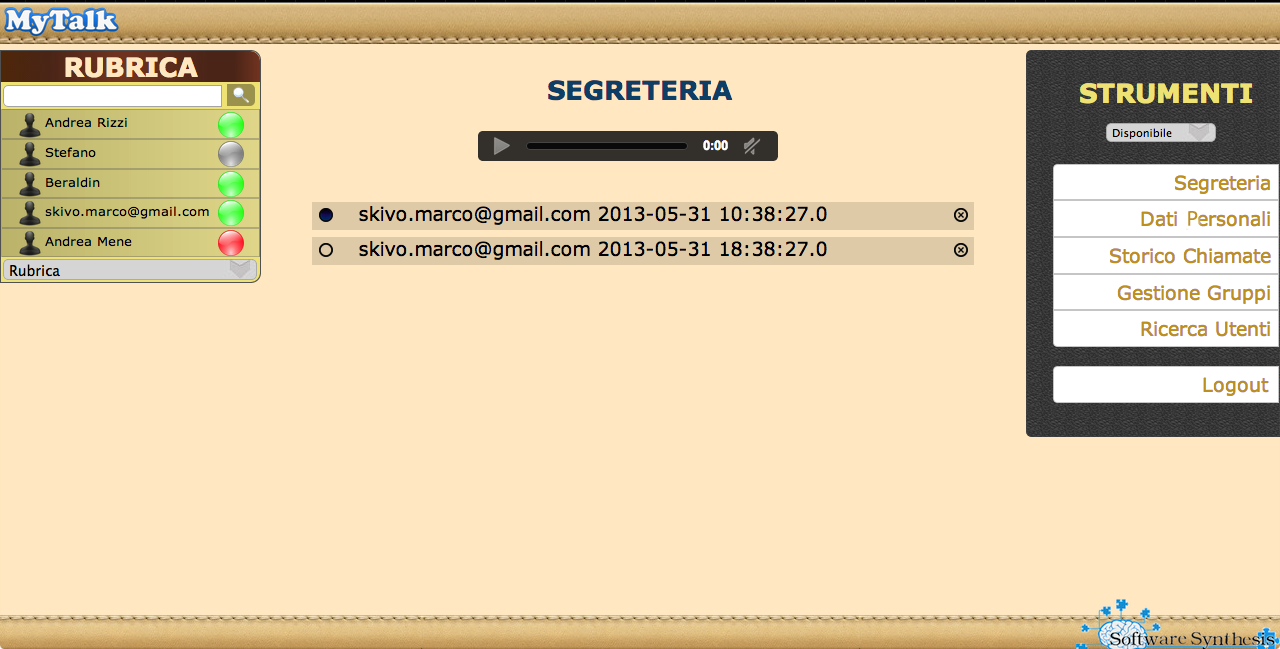
\includegraphics[width=0.8\textwidth]{manual_segreteria}
\caption{Schermata relativa alla gestione della segreteria}\label{fig:manual_segreteria}
\end{figure}

Ogni messaggio può essere ascoltato selezionandolo dalla lista dei messaggi e premendo il pulsante ``\inglese{play}''. Nel momento in cui si seleziona un messaggio, esso viene subito importato come ``visualizzato'', ma qualora si desiderasse reimpostare un messaggio già visualizzato in ``da visualizzare'', sarà sufficiente premere sull'icona vuota riportata alla sinistra del messaggio.
I messaggi vengono salvati nella memoria centrale dell'applicazione \caName{} finché l'utente non desidera eliminare esplicitamente lo stesso mediante un \textit{click} sull'icona ``\texttt{X}'' riportata alla sinistra di ogni messaggio. 
Una volta eliminato un messaggio non può essere ripristinato in alcun modo.

Invece per lasciare un messaggio in una segreteria altrui, è sufficiente premere il pulsante dell'utente (bloccato) con il quale si desidera comunicare. Quindi comparirà nell'area centrale il suo profilo e il pulsante ``Lascia un messaggio''. Premendolo comparirà la seguente schermata:

\begin{figure}[H]
  \centering
  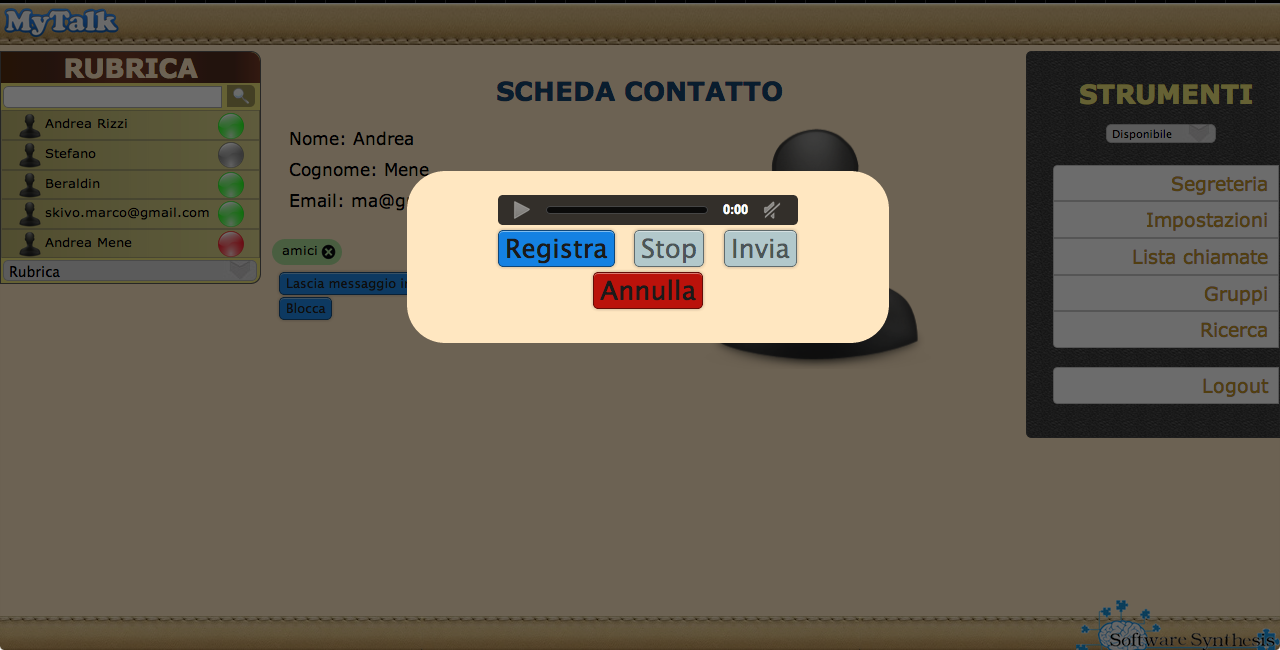
\includegraphics[width=0.8\textwidth]{manual_segreteria2}
\caption{Schermata relativa all'ascolto di un messaggio}\label{fig:manual_segreteria2}
\end{figure}

I pulsanti ``Registra'', ``Stop'' ed ``Invia'' permettono di gestire la nostra registrazione. Prima dell'invio tramite la pressione dell'omonimo pulsante, è sempre possibile annullare l'operazione usando il tasto ``Annulla''.

\clearpage
\subsection{Dati personali}
La schermata \texttt{Dati personali} è dedicata alla visualizzazione e alle modifiche dei dati del proprio \inglese{account}. Tali modifiche consentono il cambiamento dei propri dati anagrafici e la possibilità di caricare una nuova immagine da abbinare al proprio profilo, sostituendo quella (eventualmente) precedentemente associata.

\begin{figure}[H]
  \centering
  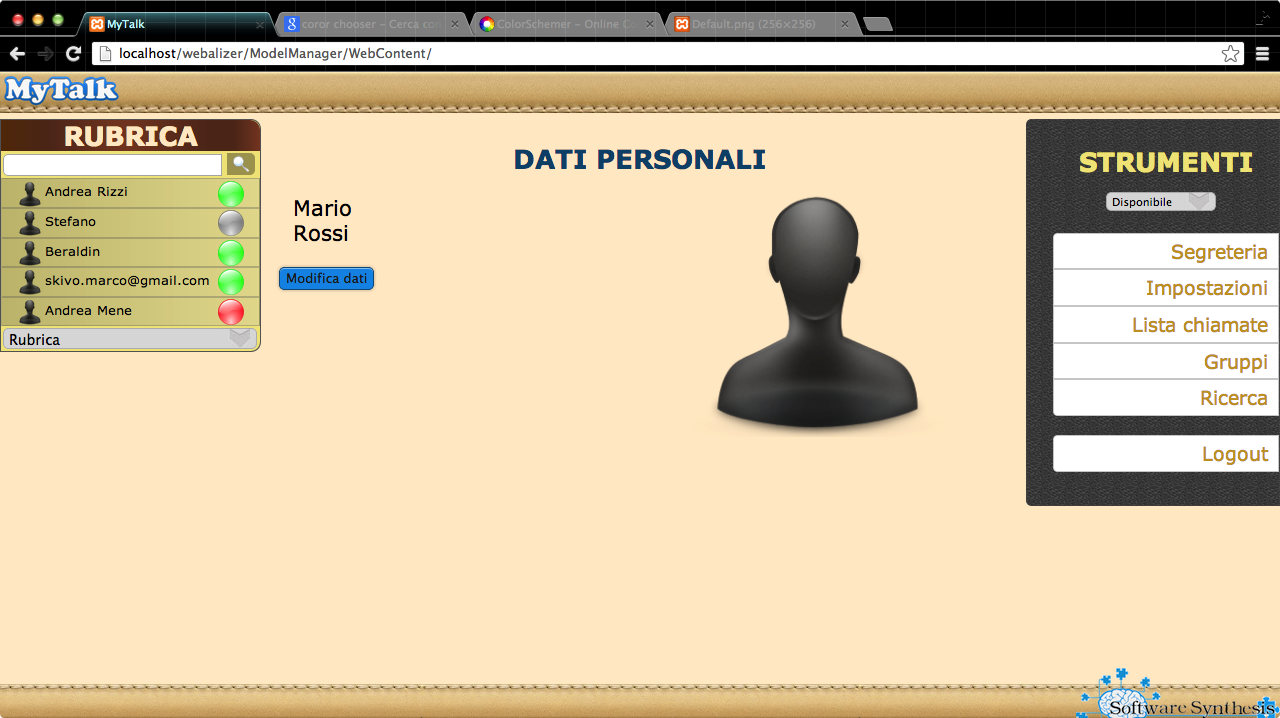
\includegraphics[width=0.85\textwidth]{manual_setting}
\caption{Schermata delle impostazioni dell'account}\label{fig:setting}
\end{figure}

\clearpage
\subsection{Storico chiamate}
Lo storico presenta una lista delle chiamate effettuate e ricevute dall'utente durante l'utilizzo di \caName{}. Ogni chiamata sarà caratterizzata da informazioni dettagliate su di essa, quali: \texttt{chiamante,destinatario,data(gg/mm/aaaa), orario d'inizio}.
Per distinguere visivamente le chiamate effettuate da quelle ricevute si fa riferimento al codice cromatico che assegna il colore \textit{verde} alle chiamate da noi effettuate e il \textit{rosso} per le chiamate ricevute. 

\begin{figure}[H]
  \centering
  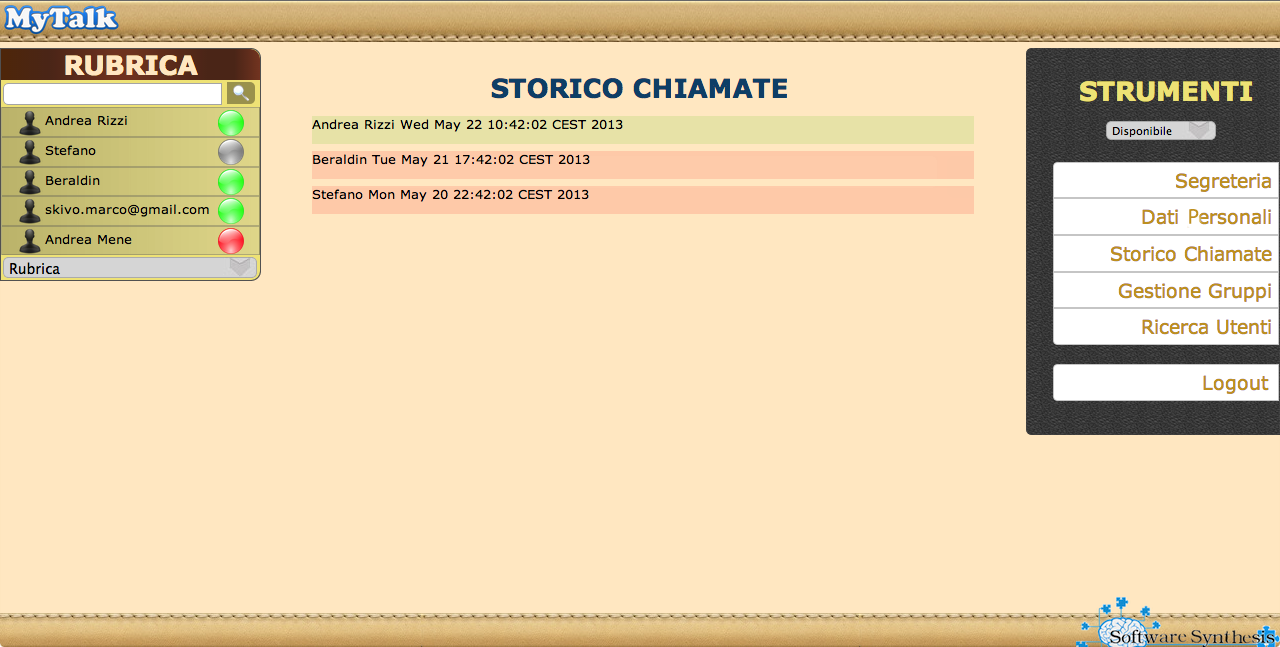
\includegraphics[width=0.85\textwidth]{manual_list}
\caption{Schermata relativa allo storico delle chiamate}\label{fig:manual_list}
\end{figure}

\clearpage
\subsection{Gruppi}
Permette, di gestire e catalogare i propri contatti mediante il loro inserimento in gruppi distinti.
La creazione di un gruppo avviene mediante il pulsante \texttt{aggiungi gruppo} e, una volta inserito il nome associato al gruppo, sarà visualizzato nella lista dei presenti.

L'inserimento di un utente in un gruppo avviene mediante il pulsante ``\texttt{+}'', selezionando tra gli utenti ancora non presenti quelli che si desidera inserire nello stesso.
Risulta inoltre possibile inserire lo stesso contatto in gruppi diversi, così da creare una classificazione più ampia possibile della classificazione di un utente in rubrica.

Si conclude specificando che l'eliminazione degli utenti dai gruppi creati avviene tramite il pulsante ``\texttt{X}'' posto a destra del rispettivo riferimento all'utente. Allo stesso modo è possibile l'eliminare i gruppi stessi: gli utenti in essi contenuti non verranno eliminati, ma semplicemente verranno deallocati dal gruppo corrispondente.

\begin{figure}[H]
  \centering
  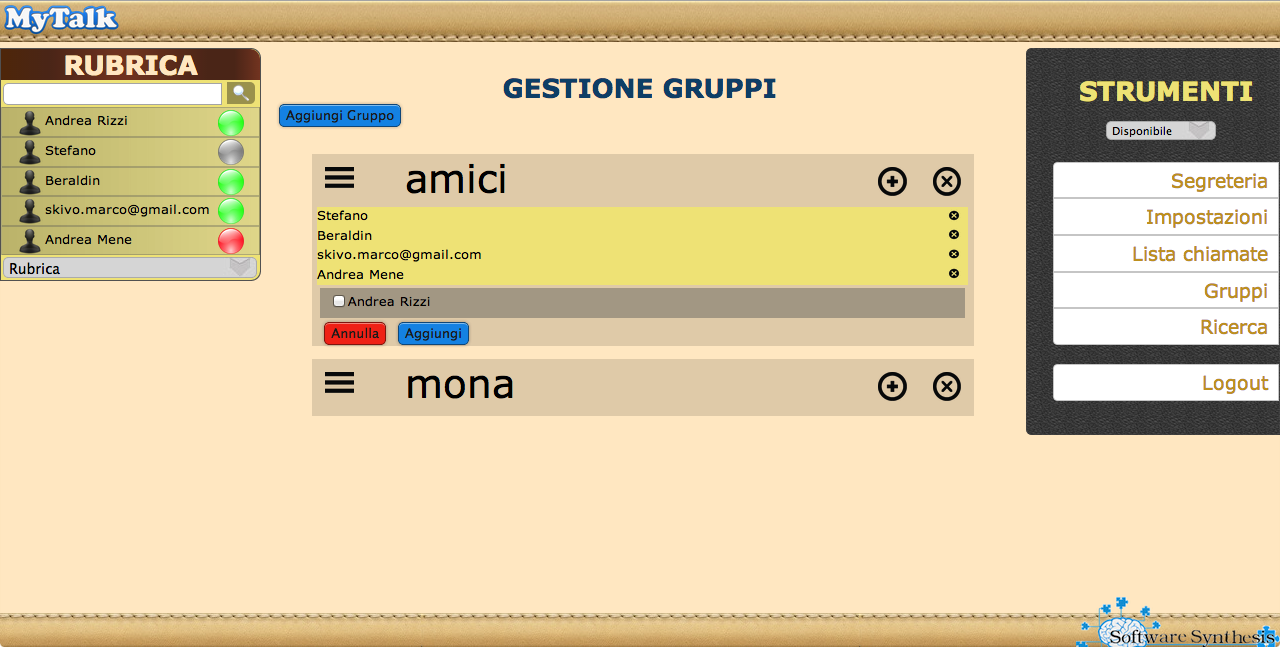
\includegraphics[width=0.85\textwidth]{manual_groups}
\caption{Schermata relativa alla gestione dei gruppi}\label{fig:manual_groups}
\end{figure}

\clearpage
\subsection{Ricerca Utenti}
Permette di aggiungere un contatto alla propria lista utenti presente in rubrica tramite una ricerca preliminare tra tutti gli utenti presenti nel sistema. Una volta individuato l'utente da aggiungere, sarà necessario premere il pulsante ``\texttt{+}'' presente a destra del nome selezionato, sarà quindi inoltrata la richiesta e automaticamente sarà aggiornata la rubrica di entrambi gli interessati.

\begin{figure}[H]
  \centering
  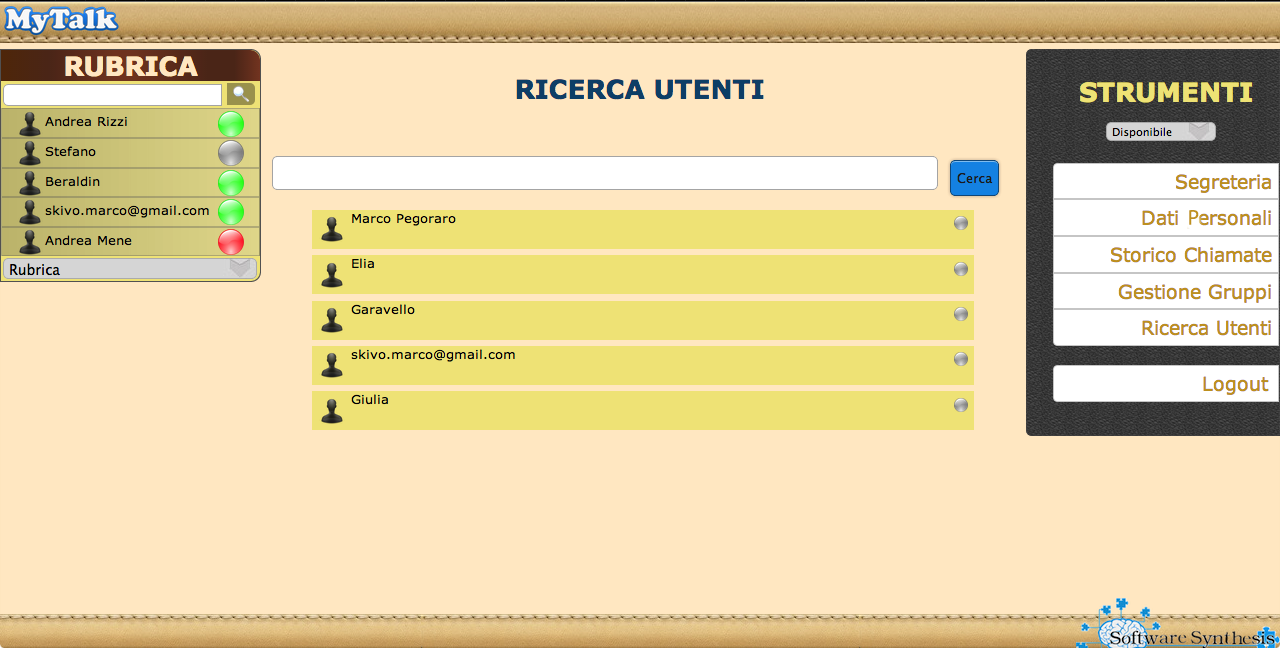
\includegraphics[width=0.85\textwidth]{manual_search}
\caption{Schermata relativa alla ricerca di un utente}\label{fig:manual_search}
\end{figure}

\subsection{Logout}

Mediante tale pulsante sarà possibile effettuare il \textit{logout} al sistema in totale sicurezza, in tale modo la sessione d'utilizzo verrà terminata e il nostro stato passerà a \texttt{non disponibile}, notificando quindi agli altri utenti l'impossibilità di comunicare con noi se non tramite l'apposita segreteria audio.

\clearpage

%\section{Errori}
%Di seguito viene riportata una tabella relativa agli errori e le relative soluzioni che il prodotto \caName{} può presentare durante il suo funzionamento.

%\begin{center}
%\rowcolors{2}{lightblue}{llightblue}\begin{longtable}{llp{.6\textwidth}}
%\toprule Codice Errore & Nome Errore  & Possibili soluzioni\\
%\midrule
%\bottomrule
%\end{longtable}
%\end{center}

\section{Glossario}
\begin{description}
\item\textbf{Account:} termine usato per identificare le credenziali d'accesso di un utente.È composto dal \textit{nome utente} e la \textit{password} impostate in fase di registrazione, nonché tutte le informazioni relative alle misure di sicurezza per il cambio password e i propri dati anagrafici.
\item\textbf{\inglese{browser}:} è un programma che consente di usufruire dei servizi di connettività in rete e di navigare sul \inglese{World Wide Web} (internet ndr.), permettendo di visualizzare i contenuti delle pagine dei siti web, specificandone l'\inglese{url} e di interagire con essi.
\item\textbf{Url:} indirizzo identificativo di ogni sito web, in modo da raggiungerlo e visualizzarlo. La barra di inserimento di tale indirizzo generalmente è posizionata nella parte superiore del \inglese{browser}.
\item\textbf{Login:} termine inglese per definire ``autenticazione''.
\item\textbf{Plugin:} è un programma non autonomo che interagisce con un altro programma per ampliarne le funzioni o offrire più servizi.
\item\textbf{Schermata Home:} schermata iniziale e principale, da essa è possibile accedere tramite uno o più passi a tutte le funzioni messe a disposizione dal prodotto.
\item\textbf{Username:} termine inglese per definire ``nome utente''. Definisce il nome con il quale l'utente viene riconosciuto da un computer, da un programma o da un \inglese{server}. In altre parole, esso è un identificativo che, insieme alla password, rappresenta le credenziali per accedere alle risorse o in un sistema.
\item\textbf{Versione sviluppatori:} versione di un programma o di un generico prodotto non ancora disponibile per l'utenza finale (\inglese{consumer}) in quanto non ancora sufficientemente  stabile o priva di malfunzionamenti. Alla correzione degli stessi generalmente viene rilasciata la versione pubblica.
\end{description}

\end{document}